\chapter{相关技术简介}
\label{cha:related-technologies}

本章介绍移动边缘计算、任务卸载、多智能体强化学习与注意力聚合的技术背景，并说明这些机制与多 UAV-MEC 决策的关系。注意力机制在本文中用于上层轨迹观测的聚合；其相对替代架构的独立收益仍须由同信息预算实验判断，不能由技术背景直接推定。

% ============================================================
\section{无人机辅助移动边缘计算技术}
\label{sec:uav-mec-technology}
% ============================================================

% ------------------------------------------------------------
\subsection{移动边缘计算概述}
\label{subsec:mec-overview}

随着物联网和智能终端设备的快速发展，计算密集型和时延敏感型应用不断涌现，对网络服务的实时性和计算能力提出了更高要求。传统的云计算架构受限于核心网络与终端设备之间的物理距离，数据传输时延难以满足低时延应用的需求。为此，欧洲电信标准化协会（ETSI）于 2014 年提出了移动边缘计算（Mobile Edge Computing, MEC）的概念\cite{etsi2019mec}，将计算和存储资源从云端下沉至网络边缘，使数据处理更加靠近终端用户。

MEC的基本架构分为三层：终端设备层、边缘服务器层和云服务器层，如图~\ref{fig:mec_architecture}~所示。终端设备层包括各类用户设备（User Equipment, UE），如智能手机、笔记本电脑、物联网传感器、监控摄像头等；边缘服务器层由部署在网络边缘的基站和边缘服务器（MEC）组成，通常与基站共址部署，提供本地化的计算和存储资源；云服务器层包含云数据中心，通过核心网络与边缘层连接，提供全局性的计算和存储资源。

在该架构下，MEC系统的工作流程包括三个关键环节：（1）任务卸载，用户设备将计算任务通过无线链路发送至就近的边缘服务器执行；（2）结果返回，边缘服务器完成计算后将结果返回给用户设备；（3）云端协同，当边缘服务器资源不足或需要全局信息时，可与云数据中心进行协同处理。这种架构设计使得终端设备可将计算任务卸载至就近的边缘服务器执行，从而显著降低传输时延、节省终端能耗、减轻核心网络带宽压力\cite{mao2017survey}。

\begin{figure}[htbp]
    \centering
    \includegraphics[width=0.85\textwidth]{docs/figures/图2-1_MEC三层架构示意图}
    \caption{移动边缘计算三层架构示意图}
    \label{fig:mec_architecture}
\end{figure}


% ------------------------------------------------------------
\subsection{任务卸载技术}
\label{subsec:offloading}

任务卸载是 MEC 系统的核心技术之一，旨在将终端设备的计算任务部分或全部转移至边缘服务器执行\cite{chen2024task}。根据卸载决策的粒度，任务卸载可分为二元卸载和部分卸载两种模式：二元卸载要求每个任务选择完全本地执行或完全卸载至边缘服务器；部分卸载则允许任务被分割为多个子任务，分别在本地和边缘服务器上并行执行。

任务卸载决策需综合考虑任务的计算量、数据量、时延要求、信道状态、边缘服务器的计算能力以及终端设备的能耗约束等因素\cite{deng2024ml}。典型的任务卸载优化问题通常需要在以下目标之间进行权衡：

（1）时延最小化。对于实时视频分析、增强现实等时延敏感型应用，最小化任务完成时间是首要目标。

（2）能耗最小化。终端设备通常由电池供电，在保证服务质量的前提下最小化终端能耗亦是重要的优化目标。

（3）时延-能耗联合优化。在实际应用中，时延和能耗往往需要同时考虑，通过加权和或约束优化的方式实现多目标平衡\cite{liu2024task}。

在多 UAV-MEC 系统中，UAV 轨迹会改变接纳范围与通信条件，卸载决策则影响已接纳请求的完成时延，两者需要协同考虑\cite{zhao2024robust}。通用 MEC 文献中的“本地执行”通常指 UE 本地计算；本文的自然覆盖仿真先由 UAV 接纳服务请求，后文卸载动作中的“本地”专指\emph{接纳 UAV 本地执行}，另可选择 MBS 或协作 UAV。深度强化学习为动态联合决策提供了一类可行的近似方法\cite{liu2024gan, zhang2024task}，但不保证求得全局最优策略。

% ------------------------------------------------------------
\subsection{无人机辅助通信与计算}
\label{subsec:uav-mec}

在这一背景下，无人机（Unmanned Aerial Vehicle, UAV）凭借灵活部署、按需覆盖与高机动性等优势，在辅助无线通信和边缘计算领域展现出显著的应用潜力\cite{zeng2016wireless}。与传统地面基站相比，UAV 具有以下优势：其一，UAV 可快速部署至目标区域，尤其适用于应急通信和临时热点覆盖场景\cite{erdelj2017help}；其二，UAV 可通过调整飞行高度和位置优化与地面用户的视距（Line-of-Sight, LoS）链路质量，提供更可靠的通信服务\cite{mozaffari2019tutorial}；其三，搭载计算资源的 UAV 可作为空中移动边缘服务器，为地面用户提供计算卸载服务\cite{hu2021uav}。

根据 UAV 在系统中承担的不同角色，UAV 辅助通信的应用场景可分为以下三类：

（1）UAV 作为空中基站。在地面基础设施受损或缺乏的场景下，UAV 可作为空中基站直接为地面用户提供通信服务。例如，在地震、洪水等自然灾害发生后，地面通信基础设施可能遭到严重破坏，此时 UAV 可快速升空建立应急通信网络，保障救援行动的通信需求\cite{erdelj2017help}。

（2）UAV 作为中继节点。当源节点与目的节点之间存在障碍物或距离过远导致直接通信困难时，UAV 可充当中继节点转发数据，扩展网络覆盖范围。这种场景在城市峡谷、山区地形等复杂环境中尤为适用。

（3）UAV 作为移动边缘服务器。近年来，将 MEC 服务器搭载至 UAV 的研究受到广泛关注\cite{hu2021uav, zhou2020latency}。在该架构下，UAV 不仅提供通信服务，还可为地面用户的计算任务提供卸载执行服务。通过联合优化 UAV 的飞行轨迹和任务卸载策略，可同时优化系统的时延和能耗性能\cite{zhang2021energy}。

上述应用场景可概括为图~\ref{fig:uav_scenarios}~所示的 UAV 辅助通信系统全景。在该系统中，宏基站作为中央通信枢纽，与各类 UAV 应用场景互联互通。UAV 既可独立承担特定任务，如大规模临时接入覆盖、物联网设备数据采集和移动边缘计算卸载，也可协同工作以实现中继转发和多机间通信。此外，UAV 还需同时服务于边缘用户和基站用户，体现了 UAV 辅助通信系统的多样性和复杂性。

\begin{figure}[htbp]
    \centering
    \includegraphics[width=0.85\textwidth]{docs/figures/图2-2_UAV辅助通信应用场景}
    \caption{UAV 辅助通信应用场景示意图}
    \label{fig:uav_scenarios}
\end{figure}

多 UAV 协作的 MEC 系统可由不同 UAV 服务不同区域或用户组，并通过调度分配计算与通信资源\cite{bai2021multi}。UAV 位置决定请求是否可被自然接纳，以及接纳后的链路条件；卸载又影响各执行节点的资源竞争。本文据此分别考察覆盖接纳和接纳后服务质量，而不预设某一种优化算法在所有场景中占优。

% ============================================================
\section{多智能体强化学习技术}
\label{sec:marl-technology}
% ============================================================

% ------------------------------------------------------------
\subsection{强化学习基础}
\label{subsec:rl}

强化学习（Reinforcement Learning, RL）作为机器学习的重要分支，旨在让智能体通过与环境交互学习最优行为策略\cite{sutton2018reinforcement}。如图~\ref{fig:rl_framework}~所示，在强化学习框架中，智能体在每个时间步 $t$ 观察环境状态 $s_t$，根据当前策略选择一个动作 $a_t$ 执行；环境接收该动作后转移至新状态，并向智能体反馈即时奖励信号 $r_t$。智能体的目标是通过不断试错学习，找到一个最优策略 $\pi^*$，使得长期交互过程中获得的累积折扣奖励最大化。

\begin{figure}[htbp]
    \centering
    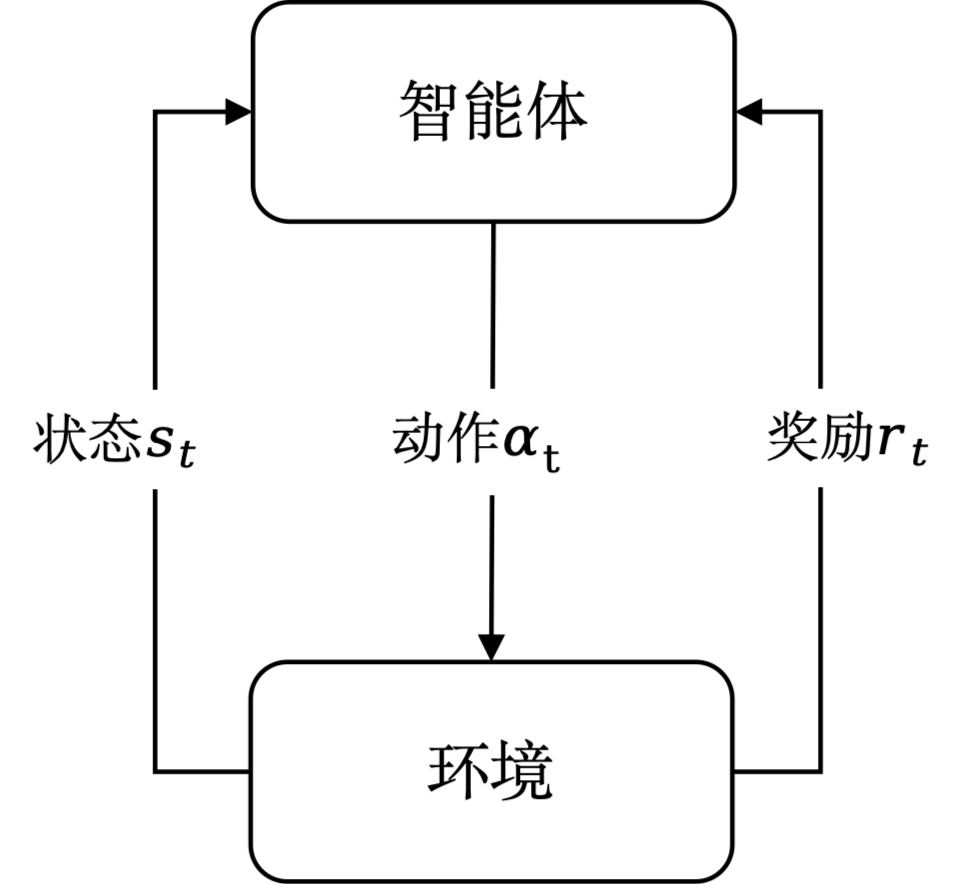
\includegraphics[width=0.6\textwidth]{docs/figures/图2-3_强化学习智能体环境交互框架}
    \caption{强化学习智能体与环境交互框架}
    \label{fig:rl_framework}
\end{figure}

强化学习问题通常被建模为马尔可夫决策过程（Markov Decision Process, MDP），可用五元组 $(S, A, P, R, \gamma)$ 描述\cite{kaelbling1996reinforcement}。其中，$S$ 为状态空间，$A$ 为动作空间，$P: S \times A \times S \rightarrow [0, 1]$ 为状态转移概率函数，$R: S \times A \rightarrow \mathbb{R}$ 为奖励函数，$\gamma \in [0, 1)$ 为折扣因子。MDP 的核心性质是马尔可夫性，即下一状态仅取决于当前状态和动作，与历史状态无关。

根据学习方式的不同，强化学习算法可分为以下几类：

（1）基于值函数的方法。通过学习状态值函数 $V(s)$ 或状态-动作值函数 $Q(s, a)$ 间接求解最优策略。典型算法包括 Q-Learning\cite{watkins1992q}和 SARSA 等。当状态空间较大或连续时，可使用深度神经网络近似值函数，如 DQN\cite{mnih2015human}。

（2）基于策略梯度的方法。直接参数化策略 $\pi_\theta(a|s)$，通过梯度上升优化策略参数 $\theta$。REINFORCE 算法\cite{williams1992simple}是策略梯度方法的经典代表，通过蒙特卡洛采样估计策略梯度。

（3）Actor-Critic 方法。结合值函数方法和策略梯度方法的优点，同时学习策略网络（Actor）和价值网络（Critic）。Actor 负责选择动作，Critic 负责评估动作的好坏，两者相互促进学习。典型算法包括 A2C、A3C 以及 DDPG\cite{lillicrap2016continuous}等。

近端策略优化（Proximal Policy Optimization, PPO）\cite{schulman2017proximal}通过截断重要性采样比率限制单次策略更新的幅度，以改善训练稳定性；广义优势估计（Generalized Advantage Estimation, GAE）\cite{schulman2015high}可在优势估计的偏差与方差之间作权衡。实际稳定性仍取决于任务和超参数设置。

上述强化学习方法主要针对单智能体场景，即系统中仅有一个决策者与环境交互。然而，在多 UAV-MEC 系统中，每架 UAV 都是一个独立的决策主体，需要在考虑其他 UAV 行为的同时做出自身决策。这种多智能体决策场景需要将强化学习扩展到多智能体框架下，即多智能体强化学习。

% ------------------------------------------------------------
\subsection{多智能体强化学习概述}
\label{subsec:marl}

多智能体强化学习（Multi-Agent Reinforcement Learning, MARL）是强化学习在多智能体系统中的自然扩展\cite{busoniu2008comprehensive}。在多智能体环境中，多个智能体同时与环境交互，每个智能体的动作都会影响环境状态和其他智能体的观察。与单智能体强化学习相比，MARL 面临以下独特挑战：

（1）非平稳性。在多智能体学习过程中，每个智能体的策略都在不断更新，这意味着从单个智能体的视角来看，环境是动态变化的，不满足马尔可夫性质。这种非平稳性使得智能体难以收敛到稳定的最优策略。

（2）信用分配问题。在协作任务中，所有智能体共享同一个全局奖励，但如何将该奖励合理地分配给每个智能体是一个困难的问题。如果不能正确地分配信用，智能体将无法判断自身行为对团队目标的贡献。

（3）可扩展性问题。随着智能体数量的增加，联合状态空间和联合动作空间呈指数增长，导致学习算法难以在可接受的时间内收敛。

根据训练和执行方式的不同，MARL 算法可分为以下三类\cite{gronauer2022multi}：

（1）集中式训练集中式执行（CTCE）。在训练和执行阶段均使用全局信息，适用于完全可观察的环境。

（2）集中式训练分散式执行（CTDE）。在训练阶段可访问全局信息（如全局状态或其他智能体的动作），在执行阶段每个智能体仅根据自身观察做出决策。该范式在实践中应用最为广泛，代表性算法包括 MAPPO\cite{yu2022surprising}、MADDPG\cite{lowe2017multi}等。

（3）分散式训练分散式执行（DTDE）。每个智能体完全独立地学习和执行，不依赖全局信息。该方法的可扩展性最好，但学习效率通常较低。

在多 UAV-MEC 系统中，CTDE 范式具有天然的适配性。在训练阶段，系统可获取全局信息（如所有 UAV 的位置、所有用户的任务状态），这有助于训练出具有全局视野的价值网络；在执行阶段，每架 UAV 仅需根据自身观察（如邻居 UAV 的位置、关联用户的任务）即可独立决策，这符合实际部署中分布式执行的需求。因此，CTDE 范式成为多 UAV-MEC 系统中 MARL 算法设计的主流选择。

根据方法论的不同，MARL 算法还可分为值分解方法和 Actor-Critic 方法两大类。值分解方法，如 QMIX\cite{rashid2018qmix}和 VDN\cite{sunehag2018value}，通过将全局 Q 函数分解为各智能体的局部 Q 函数来实现分散式执行。Actor-Critic 方法则为每个智能体维护独立的 Actor，同时使用共享的 Critic 提供全局价值评估。

% ------------------------------------------------------------
\subsection{MAPPO 算法介绍}
\label{subsec:mappo}

MAPPO（Multi-Agent Proximal Policy Optimization）是 PPO 算法在多智能体协作场景下的扩展，由 Yu 等人\cite{yu2022surprising}在 NeurIPS 2022 上系统验证了其有效性。研究表明，MAPPO 在多个主流多智能体基准任务上取得了与复杂离线策略算法相当甚至更优的性能，展现出"令人惊讶的有效性"。

MAPPO 的核心架构遵循 CTDE 范式，包含以下关键设计：

（1）共享 Critic 网络。在训练阶段，所有智能体共享一个全局 Critic 网络，该网络以全局状态或所有智能体的联合观察作为输入，输出全局价值评估。共享 Critic 使得每个智能体能够获得全局视角的价值信息，有助于缓解信用分配问题。

（2）分散式 Actor 决策。每个智能体基于其局部观测输出动作，Actor 参数可以由不同智能体共享，也可以分别维护；本文的上层实现共享一套 Actor 参数，在执行时分别输入各 UAV 的局部观测。

（3）截断重要性采样。MAPPO 继承 PPO 的截断机制，通过限制策略更新幅度保证训练稳定性。其优化目标为：

\begin{equation}
    L(\theta) = \mathbb{E}\left[\min\left(\frac{\pi_\theta(a|s)}{\pi_{\theta_{\text{old}}}(a|s)} A, \text{clip}\left(\frac{\pi_\theta(a|s)}{\pi_{\theta_{\text{old}}}(a|s)}, 1-\epsilon, 1+\epsilon\right) A\right)\right]
\end{equation}

其中，$A$ 为优势函数，$\epsilon$ 为截断参数。

MAPPO 的成功可归因于以下因素：PPO 的稳定性使训练过程不易崩溃；参数共享机制降低了样本复杂度；适当的超参数设置使 MAPPO 能在不同任务上表现出色。近年来，MAPPO 已被广泛应用于多 UAV 协作\cite{zhang2025as}、自动驾驶\cite{guo2025mappo}等场景。在多 UAV-MEC 系统中，Zhao 等人\cite{zhao2024robust}提出了基于 MAPPO 的鲁棒卸载方案，通过 Beta 分布策略处理计算和通信的不确定性。

然而，标准 MAPPO 在处理大规模智能体系统时仍面临以下挑战：

（1）观察空间维度爆炸。随着智能体数量增加，每个智能体的观察空间维度急剧增长（需包含自身状态、邻居 UAV 信息、关联用户信息等），导致策略网络难以有效学习。

（2）智能体间干扰问题。标准 MAPPO 的 Actor 网络独立处理每个智能体的观察，无法显式建模智能体之间的交互关系，导致在需要紧密协作的场景中性能受限。

（3）信息聚合效率低下。在大规模系统中，每个智能体需要处理大量冗余的观察信息，但并非所有信息都对决策同等重要，缺乏有效的信息筛选机制。

针对多智能体观测的组织问题，研究者探索了注意力聚合\cite{li2025amappo}和意图共享\cite{guo2025mappo}等设计。注意力可以对邻居和用户槽位进行加权聚合，但是否提升本文所用端到端 DSR，需要在具体协议下检验。

% ============================================================
\section{注意力机制}
\label{sec:attention}
% ============================================================

注意力机制（Attention Mechanism）能够根据查询与输入元素的关系计算加权表示\cite{vaswani2017attention}。将其用于多智能体观测时，可以采用以下建模方式；这些是结构能力，不等同于本文已经证明的性能增益：

（1）聚合固定槽位。注意力把多个邻居或用户槽位映射为聚合表示；本文仍保留固定数量的原始输入槽位，并未因注意力减少网络输入维度。

（2）建模元素间关系。注意力权重随输入变化，可表示策略对不同邻居或用户特征的相对使用程度；权重本身不能直接当作因果解释。

（3）适应观测组成变化。加权求和允许聚合表示随可见 UE 与邻居的组成变化，但其计算开销和收益仍需结合具体实现评价。

注意力机制可理解为一种加权求和操作，其中权重反映了不同输入元素对当前输出的重要程度。

给定查询向量 $Q$、键向量 $K$ 和值向量 $V$，缩放点积注意力的计算公式为：

\begin{equation}
    \text{Attention}(Q, K, V) = \text{softmax}\left(\frac{QK^T}{\sqrt{d_k}}\right)V
\end{equation}

其中，$d_k$ 为键向量的维度；缩放用于控制点积随维度增大而增长的量级，避免 softmax 过早饱和。查询与键的相似度决定各值向量的聚合权重。

多头注意力（Multi-Head Attention）进一步扩展了注意力机制的表达能力。它将查询、键和值分别通过 $h$ 组不同的线性变换投影至不同子空间，在每个子空间中独立计算注意力，最后将所有头的输出拼接并通过线性变换得到最终结果：

\begin{equation}
    \text{MultiHead}(Q, K, V) = \text{Concat}(\text{head}_1, \ldots, \text{head}_h) W^O
\end{equation}

多头注意力使模型能够同时关注不同表示子空间中的信息，增强了模型的表达能力。

在多智能体强化学习中，注意力可用于聚合其他智能体或环境元素的特征\cite{lin2024hgap}。本文上层将其用于邻居 UAV 与 UE 观测，设计动机是轨迹决策需要同时利用邻居位置和服务需求；下层是否也需要注意力，则由第三、五章的实测结果判断。

基于 Transformer 的多智能体通信方法包括建模动态有向图的 TGCNet\cite{liu2024tgcnet}、上下文感知消息生成的 CACOM\cite{li2024cacom}和邻居消息表征的 TMAC\cite{liu2025tmac}。它们说明注意力具有多种设计用途，但不能直接证明本文的注意力结构相对同信息预算替代方法更优。

% ============================================================
\section{本章小结}
\label{sec:summary-chap02}
% ============================================================

本章介绍 MEC、任务卸载、CTDE、MAPPO 和注意力聚合的基本概念。对于本文的自然覆盖系统，轨迹首先影响请求能否进入服务范围，卸载进一步影响已接纳请求是否按时完成。后续章节以实验证据评价 Attention-MAPPO 上层、无注意力学习式下层和固定快照 MC-ITR 各自的作用，而不把一种结构的理论能力预先写成端到端性能结论。
